
% Croatian Ties chapter -----------------------------------------------
\chapter*{Croatian Ties}
\addcontentsline{toc}{chapter}{Croatian Ties}

\begin{flushright}
\parbox{0.7\textwidth}{
\emph{Secrecy is the first essential in affairs of the State. \\
\hspace*{\fill}{\textperiodcentered \textperiodcentered \textperiodcentered \hspace*{0.2em} De Richelieu} } }
\end{flushright}

\noindent
Croatian Ties is chess variant which is played on 10 x 10 board,
with silver and red fields and dark silver and dark red pieces.
In algebraic notation, columns are enumerated from 'a' to 'j',
and rows are enumerated from '1' to '10'. A new piece is
introduced, Pegasus.

\clearpage % ..........................................................

\section*{Pegasus}
\addcontentsline{toc}{section}{Pegasus}

\noindent
\begin{wrapfigure}[9]{l}{0.4\textwidth}
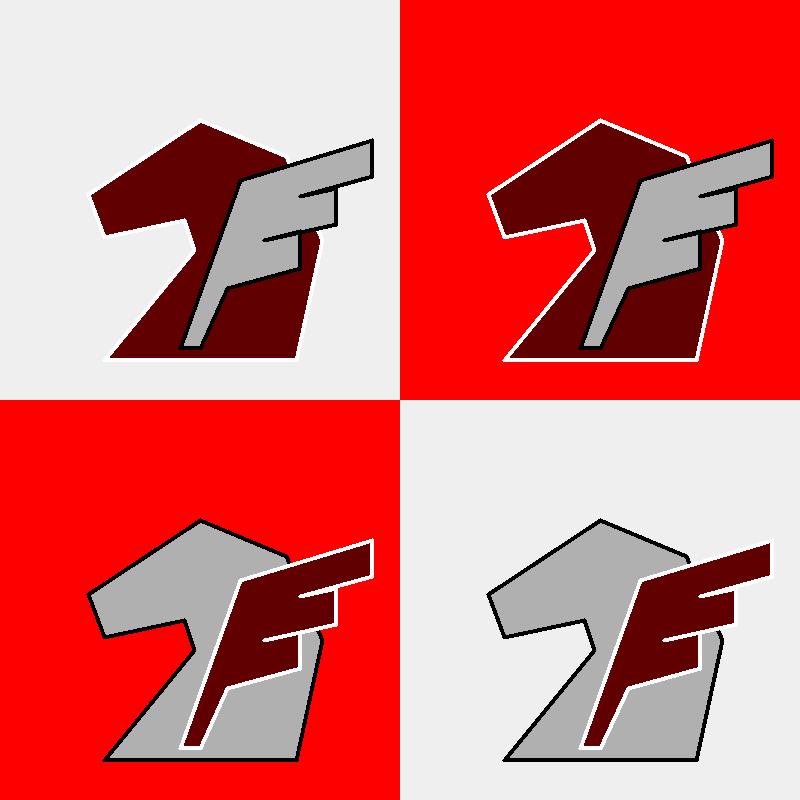
\includegraphics[width=0.4\textwidth, keepaspectratio=true]{pieces/07_pegasus.png}
\caption{Pegasus}
\label{fig:07_pegasus}
% % \centering
\end{wrapfigure}
Pegasus moves similarly to Knight, but it can continue its jumpy movement
until another piece is encountered, or it runs out of board. Note that once
in movement, Pegasus can not change its' heading.

Pegasus symbol in algebraic notation is 'G', to avoid confusion with Pawn.

\vspace{2.0\baselineskip}
\subsection*{Movement}
\addcontentsline{toc}{subsection}{Movement}

\noindent
\begin{wrapfigure}[15]{l}{0.5\textwidth}
\includegraphics[width=0.5\textwidth, keepaspectratio=true]{examples/04_move_pegasus_initial.png}
\caption{Pegasus initial step}
\label{fig:04_move_pegasus_initial}
% % \centering
\end{wrapfigure}
In the example on the left we have Pegasus with all valid initial moves marked.
These all are the same as valid moves for Knight. Pegasus' movement is not hampered
by piece if it's placed on any unmarked field. Pegasus can "jump" over it just as
Knight would.

\clearpage % ..........................................................

\noindent
\begin{figure}[!h]
% \begin{figure}[!t]
\includegraphics[width=1.0\textwidth, keepaspectratio=true]{examples/04_move_pegasus_direction.png}
\caption{Pegasus move direction}
\label{fig:04_move_pegasus_direction}
% \centering
\end{figure}

Once direction is chosen Pegasus can continue its' movement performing one jump
after another in order from nearest field to furthest. Here, this is marked
with green arrows. Accessible fields are marked 1 to 4, in order of accessibility,
from nearest to furthest. Again, once direction is chosen it can't be changed anymore.
For instance, after reaching field 2 it's not allowed to change direction to 2f (or
any other greyed-out arrow).

\clearpage % ..........................................................

\subsection*{New terms}
\addcontentsline{toc}{subsection}{New terms}

\noindent
% \begin{figure}[t]
\begin{figure}[!h]
\vspace{-1.0\baselineskip}
\includegraphics[width=1.0\textwidth, keepaspectratio=true]{examples/04_move_pegasus_step_ply.png}
\caption{Step-fields, capture-fields, ply}
\label{fig:04_move_pegasus_step_ply}
% \centering
\end{figure}

Above, field 3 is chosen as destination for Pegasus' movement. Move along arrow is a step.
Field at which arrow points to is a step-field. Here, each step-field is also capture-field,
Pegasus would be able to capture opponent's piece on it. Completed movement of Pegasus,
from its' starting position to its' destination field 3 is a ply.

\clearpage % ..........................................................

\subsection*{Movement (cont.)}
\addcontentsline{toc}{subsection}{Movement (cont.)}

\noindent
\begin{figure}[!h]
% \begin{figure}[!t]
\vspace{-1.2\baselineskip}
\includegraphics[width=1.0\textwidth, keepaspectratio=true]{examples/04_move_pegasus.png}
\caption{Pegasus moves}
\label{fig:04_move_pegasus}
% \centering
\end{figure}

Pegasus can "jump" over pieces on non-step-fields, Rooks in example above. Numbers
here enumerate directions of movement. Own piece on step-field stops Pegasus at
preceding step field, see direction 2. Opponent's piece on step-field can be captured.
Just as with any other piece that would finish the move, meaning Pegasus would have to
stop at captured step-field, see direction 1.

\clearpage % ..........................................................

\section*{En passant}
\addcontentsline{toc}{section}{En passant}

\noindent
\begin{wrapfigure}[17]{l}{0.3\textwidth}
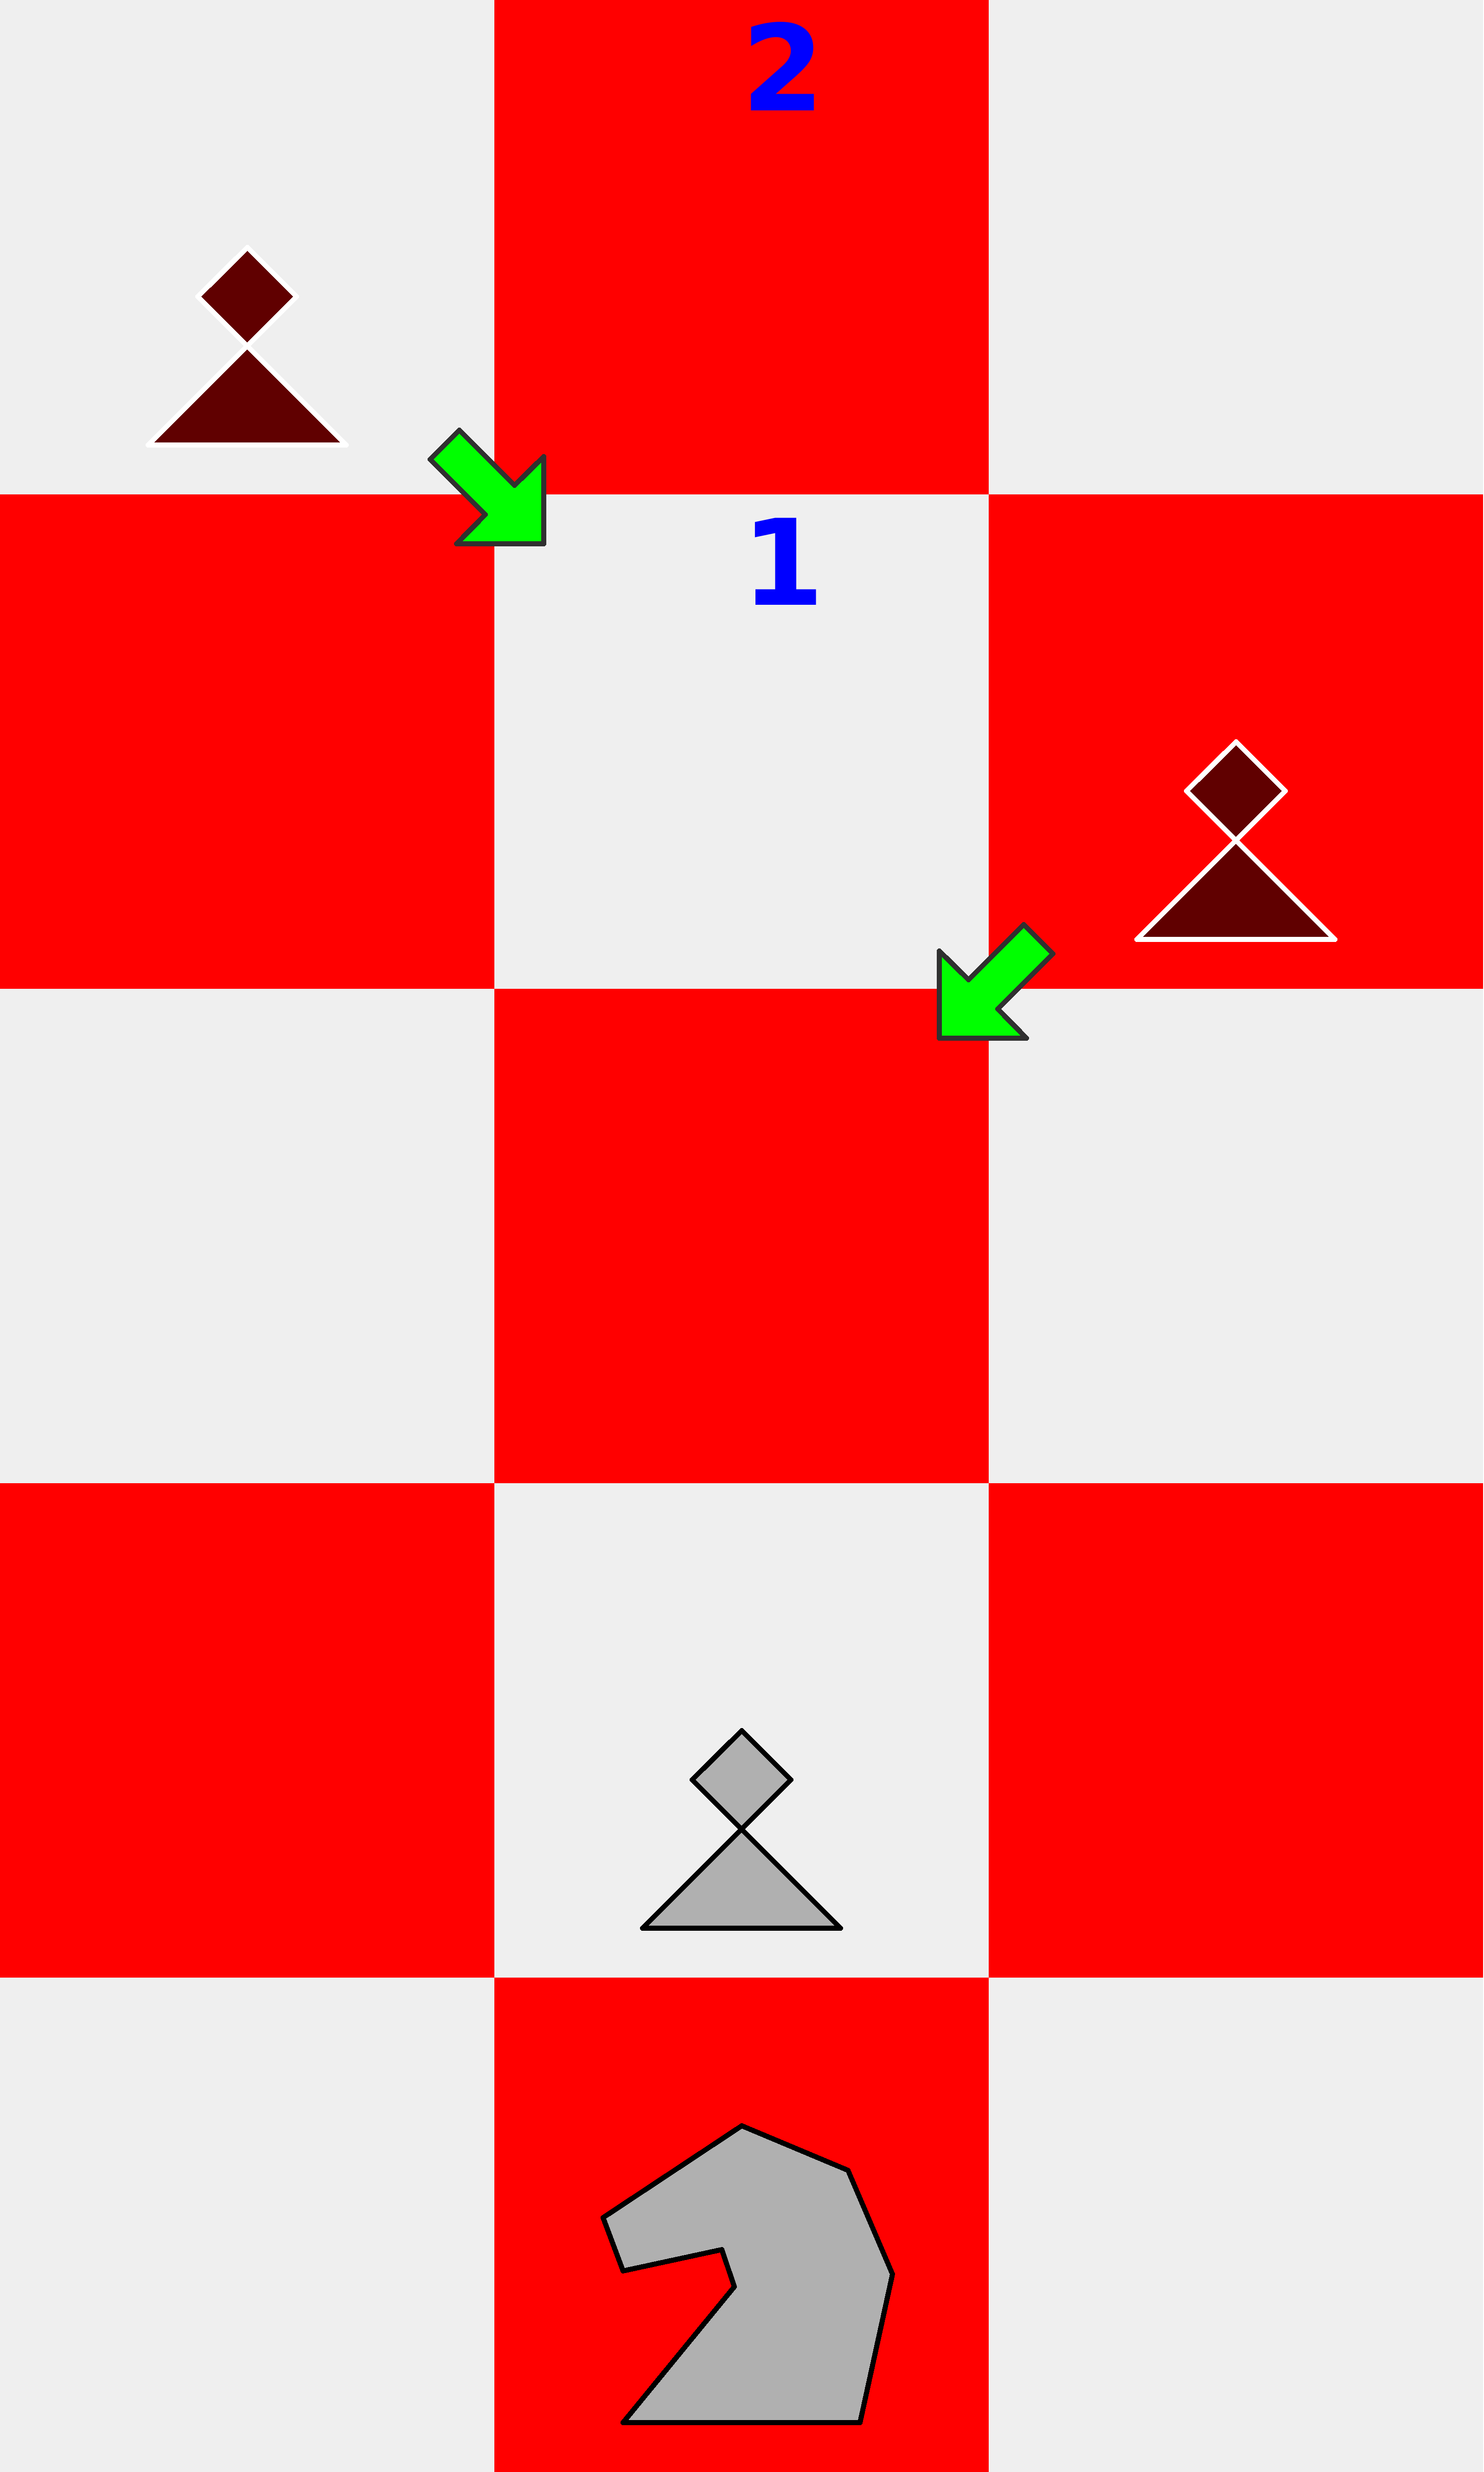
\includegraphics[width=0.3\textwidth, keepaspectratio=true]{en_passants/04_croatian_ties_en_passant.png}
\caption{En passant}
\label{fig:04_croatian_ties_en_passant}
% % \centering
\end{wrapfigure}
En passant is identical to one in Classic Chess, only difference is that Pawn can now
move longer on initial turn, up to 3 fields in this instance. As expected, all passed-by
opponent's Pawns also gain en passant opportunity.

Passed-by Pawns are those which had field under their attack passed over by opponent's Pawn
on its' initial turn, if that move was at least 2 fields long.

For example, on the left, if light Pawn's initial move was of maximum length both dark Pawns
would have en passant opportunity. Naturaly, if initial move was only to field marked 1, only
dark Pawn on the right would gain en passant opportunity.

\clearpage % ..........................................................

\section*{Castling}
\addcontentsline{toc}{section}{Castling}

Castling is essentially the same as it is in Classical Chess, only real difference is that
King can move either 2 or 3 fields across. All other constraints from Classical Chess still
applies, described in detail here \\
\href{https://en.wikipedia.org/wiki/Castling}{https://en.wikipedia.org/wiki/Castling}.

\noindent
\begin{figure}[!h]
% \begin{figure}[!t]
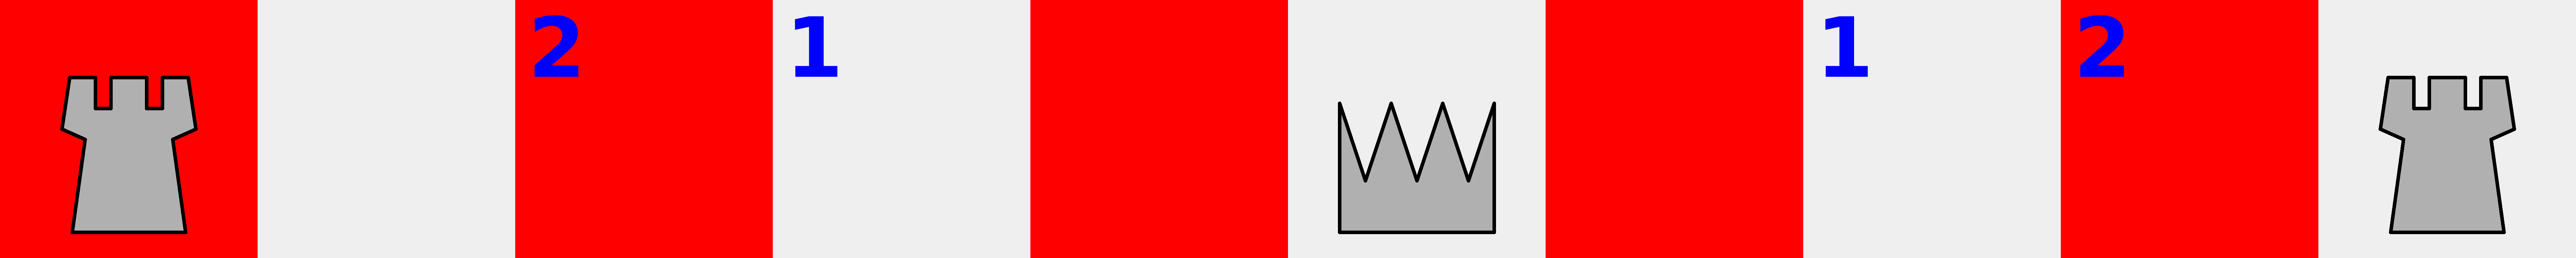
\includegraphics[width=1.0\textwidth, keepaspectratio=true]{castlings/04_croatian_ties_castling.png}
\caption{Castling}
\label{fig:04_croatian_ties_castling}
% \centering
\end{figure}

In example above, all valid King's castling moves are numbered. Regardless if King performs
long or short castling move, Rook would always end up on the opposite side of King on the
field immediately next to it, i.e. closer to center.

\noindent
\begin{figure}[!h]
% \begin{figure}[!t]
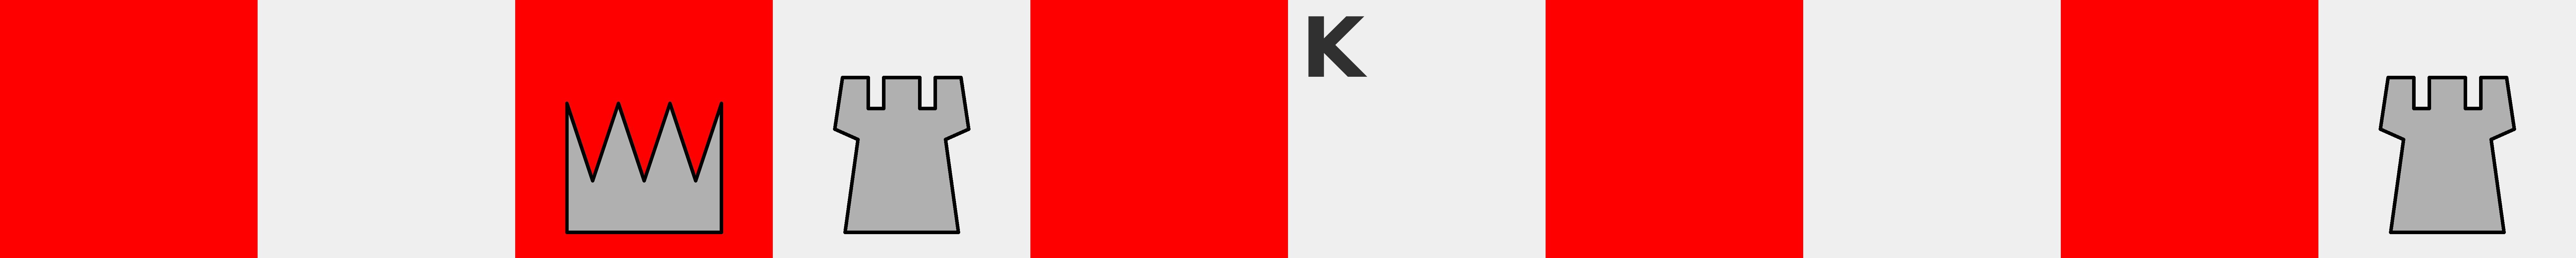
\includegraphics[width=1.0\textwidth, keepaspectratio=true]{castlings/long_left/04_croatian_ties_castling_long_left.png}
\caption{Castling long left}
\label{fig:04_croatian_ties_castling_long_left}
% \centering
\end{figure}

In this example King was castling long to the left. Initial King's position is marked with "K".
After castling is finished, left Rook ends up at field immediately on the right to the King.

\clearpage % ..........................................................

\section*{Initial setup}
\addcontentsline{toc}{section}{Initial setup}

Compared to initial setup of Classical Chess, Pegasus is inserted between Rook and Knight
symmetrically, on both sides of chess board. This can be seen in the image below:

\noindent
% \begin{figure}[t]
\begin{figure}[h]
\includegraphics[width=1.0\textwidth, keepaspectratio=true]{boards/04_croatian_ties.png}
\caption{Croatian Ties board}
\label{fig:04_croatian_ties}
% \centering
\end{figure}

\clearpage % ..........................................................
% ----------------------------------------------- Croatian Ties chapter
